This system feeds a song and its metadata first into a feature extractor. This runs simple signal processing techniques to extract features about each sample in the song that more closely related to real world values that might influence the way a human would hear it. It is then fed into a step file parser. This combines the song data is the stepmania data to label each piece of data for training. This labeled data is then used to train the neural network. The neural network determines where beats should go. This data is finally fed into a step file creator that translates the labeled data into a format that can be read by the stepmania game.
\begin{center}
	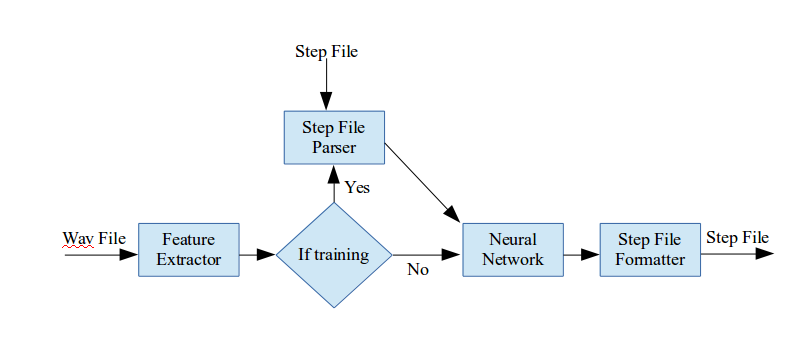
\includegraphics[scale=0.55]{data-flow.png}
\end{center}
